\documentclass[a4paper]{scrartcl}
\usepackage[ngerman]{babel}
\usepackage[utf8]{inputenc}
\usepackage[T1]{fontenc}
\usepackage{lmodern}
\usepackage{amssymb}
\usepackage{amsmath}
\usepackage{enumerate}
\usepackage{scrpage2}\pagestyle{scrheadings}
\usepackage{tikz}

\newcommand{\titleinfo}{Hausaufgaben zum 10. Mai 2012}

\title{\titleinfo}
\author{Elena Noll, Sven-Hendrik Haase, Arne Struck}
\date{\today}
\ihead{EN, SHH, AS}
\chead{\titleinfo}
\ohead{\today}
\setheadsepline{1pt}
\newcommand{\qed}{\quad \square}

\begin{document}
\maketitle

\begin{enumerate}

\item[\textbf{1.}]
\begin{enumerate}[(i)]

\item
\begin{align}
f(x) &= \frac{1}{\sqrt[4]{x^5}} * \sqrt[3]{\sqrt{x^7}} \\
&= x^{-\frac{5}{4}} * x^{\frac{7}{6}}\\
&= x^{-\frac{1}{12}}\\  	 
f'(x) &= -\frac{1}{12} x^{-\frac{13}{12}}
\end{align}
\item
\begin{align}
f(x) &= \sin(x^2) \\
f'(x)&= 2x*\cos(x^2)
\end{align}
\item
\begin{align}
f(x) &= \sin^2(x) \\
&= \sin(x)*\sin(x) \\
f'(x) &= 2*\sin(x)*d \sin(x)\\
&= 2*\sin(x)*\cos(x)
\end{align}
\item
\begin{align}
f(x) &= \sin(x)*\cos(x)\\
f'(x) &= (\sin(x)*\cos(x))'\\
&= (\sin(x)*-\sin(x)+\cos(x)*\cos(x)\\
&= -\sin^2(x)+\cos^2(x)
\end{align}
\item
\begin{align}
f(x) &= \arcsin(\sqrt{x}) \\
f'(x) &= \frac{1}{\sqrt{1-\sqrt{x^2}}} \\
f(x) &= \frac{1}{\sqrt{1-x}}
\end{align}
\item
\begin{align}
f(x) &= (x^3-1)^{\arctan(x)} \\
&= e^{\ln((x^3-1)^{\arctan (x)}} \\
&= e^{{\arctan (x)}*\ln((x^3-1)}\\
f'(x) &= e^{{\arctan (x)}*\ln((x^3-1)} * (\frac{1}{1+x^2}*\ln(x^3-1)+\arctan(x)*\frac{1}{x^3-1}*3x^2)\\
&= (x^3-1)^{\arctan(x)}*(\frac{ln(x^3-1)}{1+x^2}+\frac{3x^2*\arctan(x)}{x^3-1}
\end{align}
\end{enumerate}


\item[\textbf{2.}]
Definitionsbereich: \((-\infty,\infty)\)\\
Ableitungen:\\

\(f'(x)\):
\begin{align}
f'(x)&=2*\frac {(1+x^2)*1-f'(1+x^2)*x} {(1+x^2)^2}\\
&=2*\frac {1+x^2-2x-x} {(1+x^2)^2}\\
&=-2\frac {(x^2-1)} {(x^2+1)^2}
\end{align}

\(f''(x)\):
\begin{align}
&f''(x)=\frac {4x(x^2-3)} {(x^2+1)^3}
\end{align}

Nullstellen:\\
\(f(x)\): \(x = 0\) (einfach zu sehen durch einsetzen)\\
\(f'(x)\): \(x = 1 \vee x = -1\) (einfach zu sehen durch einsetzen)\\
\(f''(x)\): \(x = 0 \vee x = -\sqrt 3 \vee x = \sqrt 3\)

Limes:\\
\[\lim_{x \to \infty} f(x) = \lim_{x \to \infty} \frac {2x} {x^2+1} = 0\]
\[\lim_{x \to -\infty} f(x) = \lim_{x \to -\infty} \frac {2x} {x^2+1} = 0\]
\[\lim_{x \to 0} f(x) = \lim_{x \to 0} \frac {2x} {x^2+1} = 0\]

Bereiche:\\
\(f(x) < 0 \forall x \in (-\infty,0)\)\\
\(f(x) > 0 \forall x \in (0,\infty)\)

\(f'(x) < 0 \forall x \in (-\infty,-1)\)\\
\(f'(x) > 0 \forall x \in (-1,1)\)
\(f'(x) < 0 \forall x \in (1,\infty)\)


\(f''(x) < 0 \forall x \in (-\infty,-\sqrt 3)\)\\
\(f''(x) > 0 \forall x \in (-\sqrt 3,0)\)\\
\(f''(x) < 0 \forall x \in (0, \sqrt 3)\)\\
\(f''(x) > 0 \forall x \in (\sqrt 3, \infty)\)

Maxima:\\
\(f'(1) = 1\) und \(f''(1) < 0\) also liegt hier ein Minimum von f(x).\\
\(f'(-1) = -1\) und \(f''(-1) > 0\) also liegt hier ein Maximum von f(x).

Asymptoten:\\
Es sind keine Asymptoten vorhanden. Das kann auch gezeigt werden:
\[\lim_{x \to \infty} \frac {f(x)} x = \lim_{x \to -\infty} \frac {f(x)} x = \infty\]

Funktionswerte:\\
\begin{tabular}{r|c|c|c|c|c|c|c|c|c}
x & -20 & -10 & -5 & -1 & 0 & 1 & 5 & 10 & 20\\
\hline
f(x) & -0.0997506 & -0.19802 & -0.19802 & -1 & 0 & 1 & 0.384615 & 0.19802 & 0.0997506
\end{tabular}

Skizze:\\
\hspace*{-1.5in}
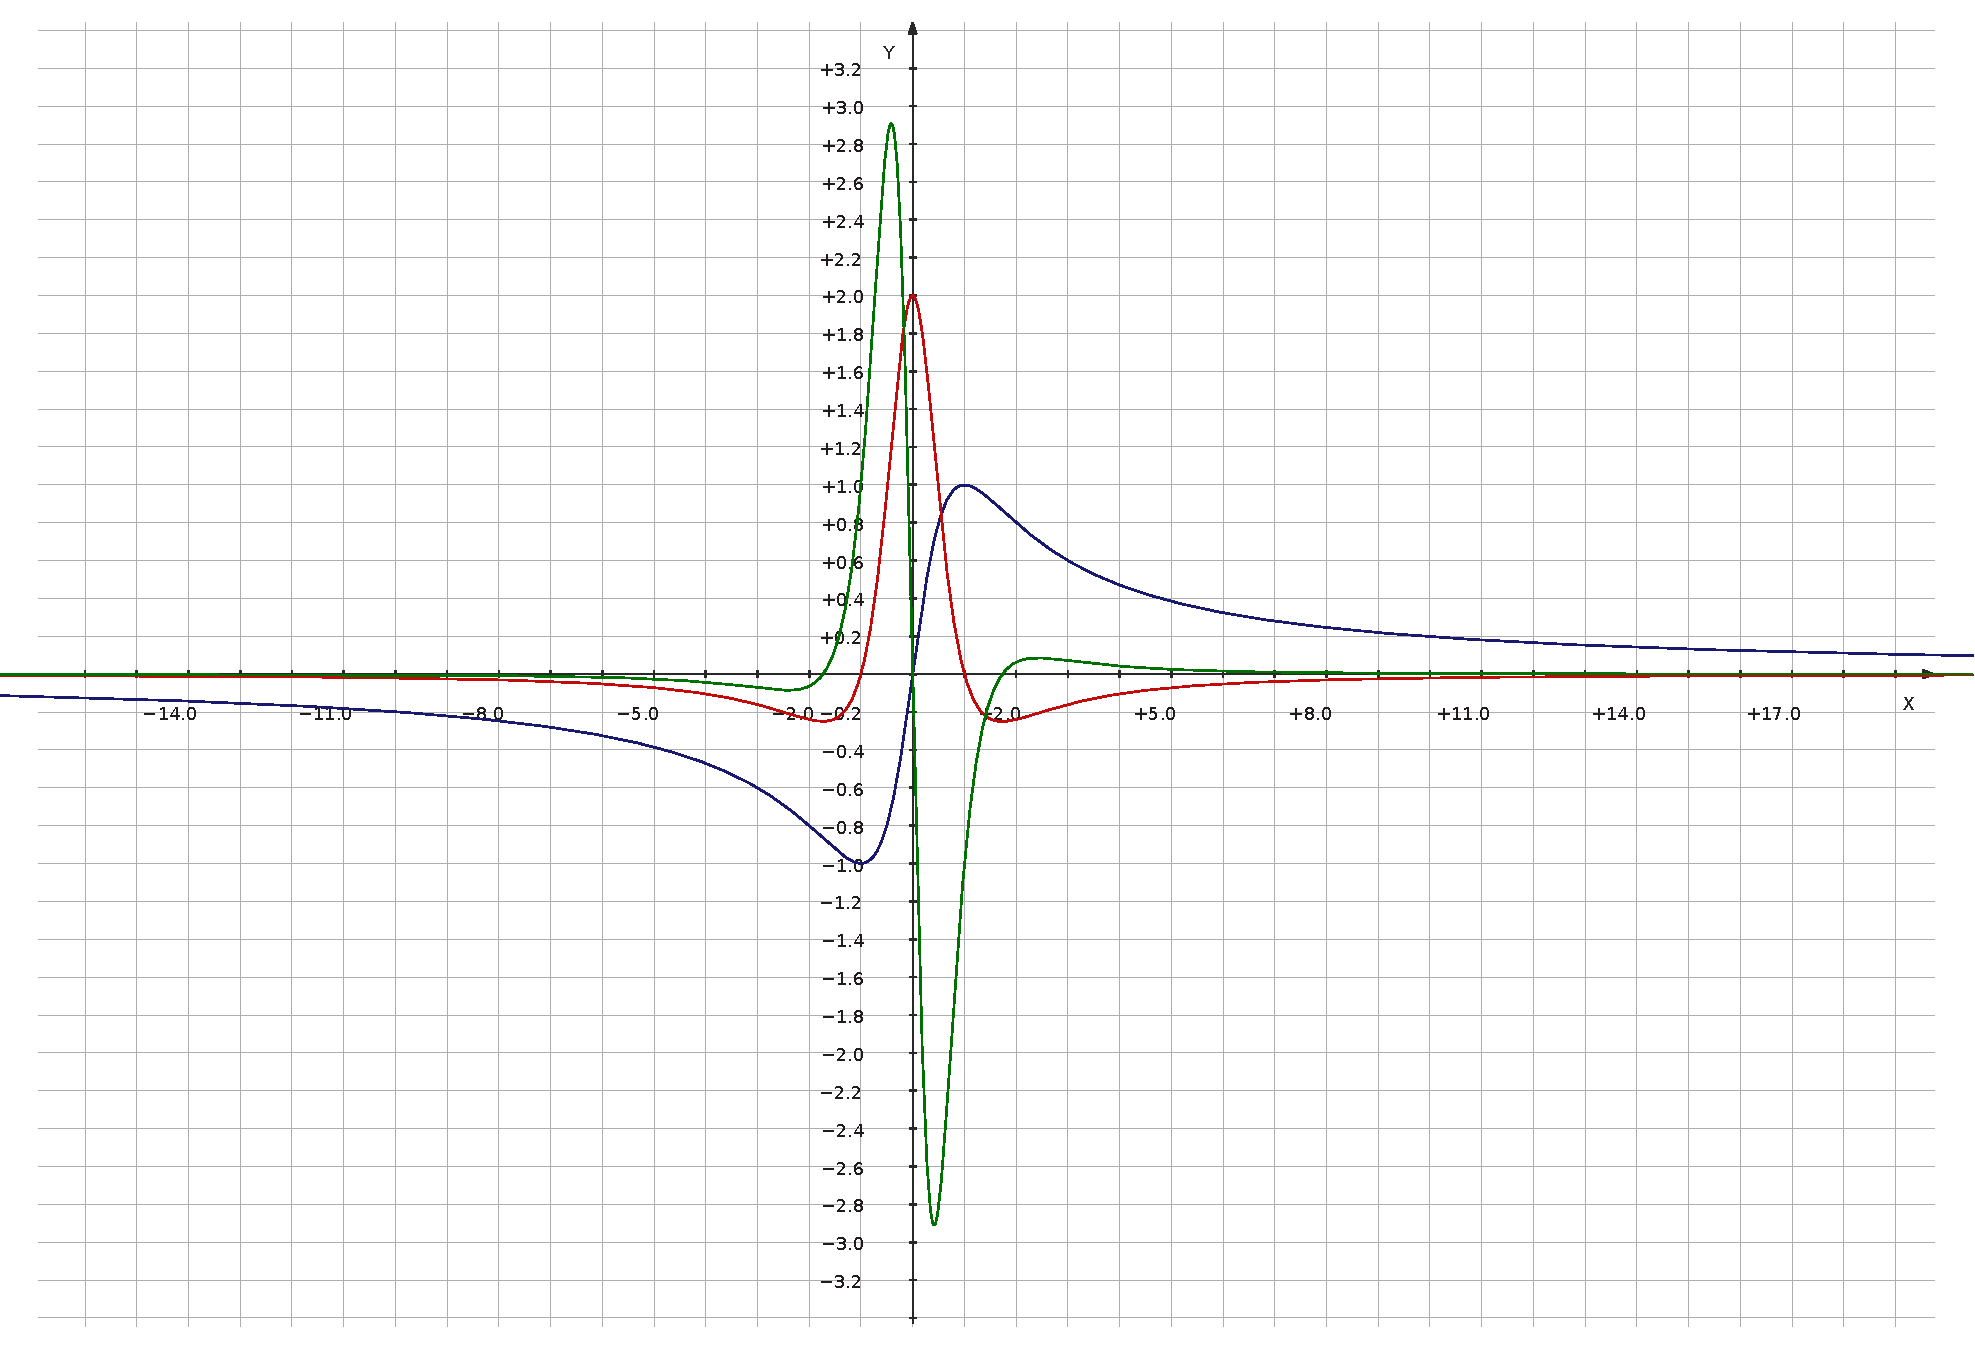
\includegraphics[scale=0.6]{Homework-2012-05-10-2.pdf}\\
Blau: \(f(x)\)\\
Rot: \(f'(x)\)\\
Grün: \(f''(x)\)


\
\item[\textbf{3.}] 

\ 

\(f:[1,2]\rightarrow \mathbb{R} \)  \\
\(f(x)= x^4-5x^2+5x-\frac{5}{2}\) \\ 
\(f'(x)= 4x^3-10x+5\)  \\
\(f''(x)= 12x^2-10x+4\)  \\

Bedingungen: \\
\((1) f'(x) \neq  0 : \forall x \in [1,2]\) : \\
\begin{center}
\begin{align}
&f'(1)= 4-10+5=-1 \\
&f'(2)= 4*2^3-10*2+5=17  \\
\end{align}
\end{center}
Da f'(1) < 0 und f'(2) > 0, Polynome stetig sind und somit ein \(x \in [1,2]\) 0 sein muss, ist die 1. Bedingung für die Anwendung des Newtonverfahrens verletzt. 

\end{enumerate}
%Ende aller Aufgaben
\end{document}

